\documentclass[11pt]{article}
\usepackage[letterpaper, scale=0.85]{geometry}
\usepackage{graphicx}
\usepackage{amsmath}
\usepackage{enumerate}
\usepackage{url}
\usepackage{caption}
\usepackage{booktabs}
\usepackage[dvipsnames]{xcolor}

\usepackage{fancyvrb}

\RecustomVerbatimCommand{\VerbatimInput}{VerbatimInput}%
{fontsize=\footnotesize,
 %
 frame=lines,  % top and bottom rule only
 framesep=2em, % separation between frame and text
 rulecolor=\color{Gray},
 %
 label=\fbox{\color{Black}data.txt},
 labelposition=topline,
 %
 commandchars=\|\(\), % escape character and argument delimiters for
                      % commands within the verbatim
 commentchar=*        % comment character
}

\setlength{\parindent}{0pt}
\begin{document}

\author{Radhika Anand}
\title{STA663 \\Infinite Latent Feature Models and the Indian Buffet Process}
\date{\today}
\maketitle

\section{Outline}
\subsection{Definition of the Indian Buffet Process}

In the Indian buffet process, N customers enter a restaurant one after another. Each customer encounters a buffet consisting of infinitely many dishes arranged in a line. The first customer starts at the left of the buffet and takes a serving from each dish, stopping after a Poisson($\alpha$) number of dishes. The ith customer moves along the buffet, sampling dishes in proportion to their popularity, taking dish k with probability $mk/i$ , where mk is the number of previous customers who have sampled that dish. Having reached the end of all previous sampled dishes, the ith customer then tries a Poisson($\alpha$/$i$) number of new dishes.


\subsection{Steps}

1) Start by defining a probability distribution over equivalence classes of binary matrices with a finite number of rows and an unbounded number of columns. This distribution is suitable for use as a prior in probabilistic models that represent objects using a potentially infinite array of features\\

2) Next we see that the Indian Buffet Process is a simple generative process that results in the same distribution (as described in previous step) over equivalence classes because IBP has finite number of objects (people) and infinite number of features (dishes)\\

3) We then define a Gibbs Sampler for models using this concept of IBP\\

4) Further, to illustrate how IBP can be used as a prior in models for unsupervised learning, we derive and test a linear-Gaussian latent feature model in which the features are binary\\

5) We start with a finite realization and then take the infinite limit\\

\section{Algorithm}
1) We use Gamma prior for $\alpha$
$$
\alpha \sim Gamma(1,1)
$$\\

2) Prior on Z is obtained by IBP (after taking the infinite limit) as:
$$
P(z_{ik}=1|\textbf{z}_{-i,k}) = \frac{m_{-i,k}}{N}
$$
where ${z}_{-i,k}$ is the set of assignments of other objects, not including i, for feature k, and
${m}_{-i,k}$ is the number of objects possessing feature k, not including i.\\

3) Likelihood is given by
\begin{equation}
P(X|Z,\sigma_X,A) = \frac{1}{(2 \pi \sigma_x^2)^{ND/2}}exp(-\frac{1}{2\sigma_X^2}tr((X-ZA)^T(X-ZA)))
\end{equation}
where Z is the binary feature matrix and A is the weight matrix. $\sigma_X$ and $\sigma_A$ are the respective noise terms.
Next, we integrate out A to get $P(X|Z,\sigma_X,\sigma_A)$.\\

4) Using this likelihood and the prior given by IBP, full conditional posterior for Z can be calculated as:
$$
P(z_{ik}|X,Z_{-(i,k)},\sigma_X,\sigma_A) \propto  P(X|Z,\sigma_X,\sigma_A) * P(z_{ik}=1|\textbf{z}_{-i,k})
$$\\

5) Now, to sample the number of new features for observation $i$, we use a truncated distribution, computing probabilities for a range of values $K_1^{(i)}$ up to an upper bound. The prior on number of features is given by $Poisson(\frac{\alpha}{N})$.
Using this prior and the likelihood, we sample the number of new features.\\

6) Conditional posterior for $\alpha$ is given by:
$$
P(\alpha|Z) \sim Gamma(1+K_+,1+\sum_{i=1}^{N} H_i)
$$
where $H_N$ is the Nth harmonic number given by $H_N=\sum_{j=1}^{N} 1/j$\\

7) We now run the Gibbs Sampler using these full conditionals\\

8) To update $\sigma_X$ and $\sigma_A$, we use MH algorithm as follows:
\begin{eqnarray}
\epsilon \sim Uniform(-.05,.05)\\
\sigma_X^{*} =  \sigma_X +\epsilon\\
\sigma_A^{*} =  \sigma_X +\epsilon\\
\end{eqnarray}

\VerbatimInput{profiling.txt}

\begin{table}[ht]
\centering
\caption{Times for likelihood function \label{time_like}}
\begin{tabular}{lr}
\toprule
{} &  Time (in secs) \\
\midrule
Old Likelihood &        0.161613 \\
New Likelihood &        0.147949 \\
\bottomrule
\end{tabular}

\end{table}

\begin{table}[ht]
\centering
\caption{Times \label{time}}
\begin{tabular}{lr}
\toprule
{} &  Time (in secs) \\
\midrule
Naive      &      343.536284 \\
Optimized  &      296.065528 \\
Cythonized &      299.767935 \\
\bottomrule
\end{tabular}

\end{table}

\begin{figure}
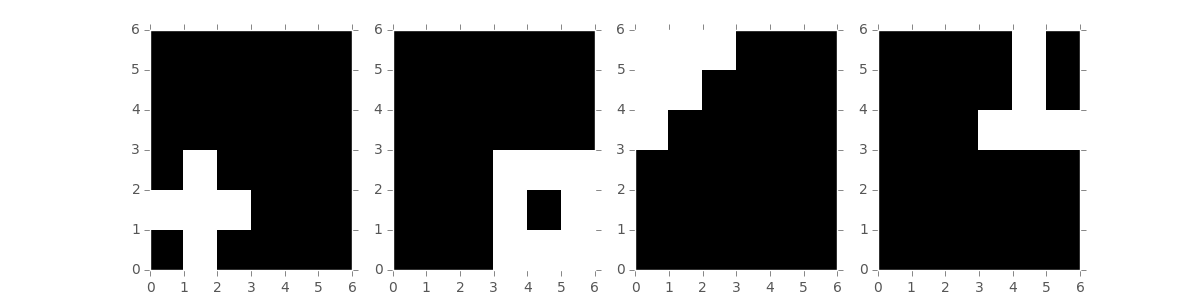
\includegraphics[width=\linewidth]{data_files/features.png}
\caption {Main features used to simulate data}
\label{fig:feat}
\end{figure}

\begin{figure}
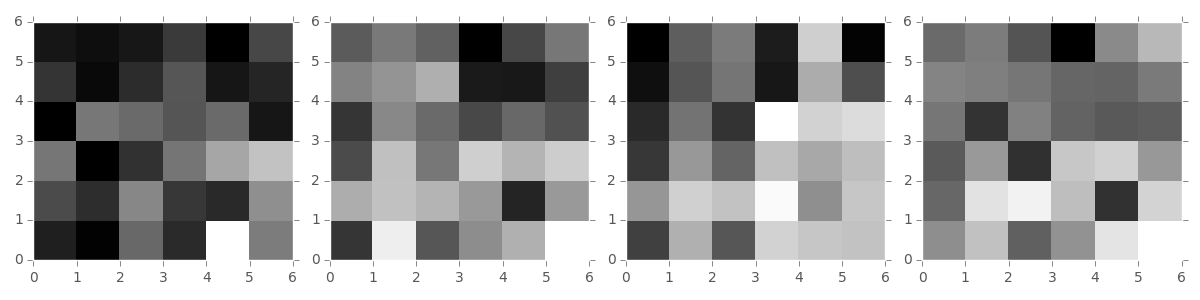
\includegraphics[width=\linewidth]{data_files/data.png}
\caption {Simulated data}
\label{fig:data}
\end{figure}

\begin{figure}
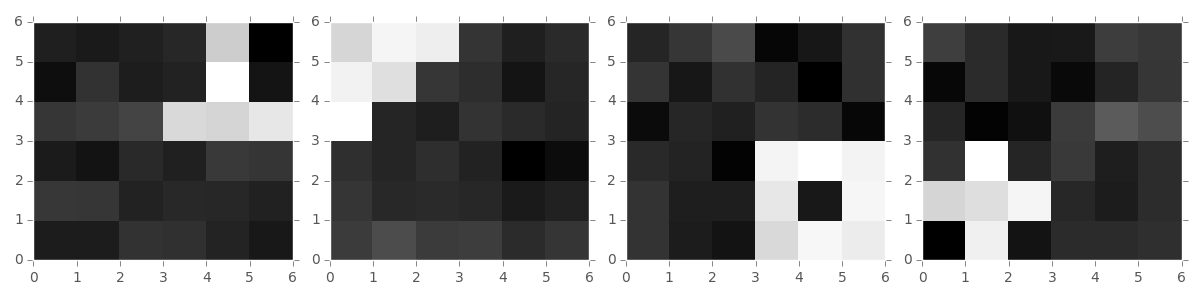
\includegraphics[width=\linewidth]{data_files/detected_features.png}
\caption {Features detected by code}
\label{fig:dat}
\end{figure}

\begin{figure}
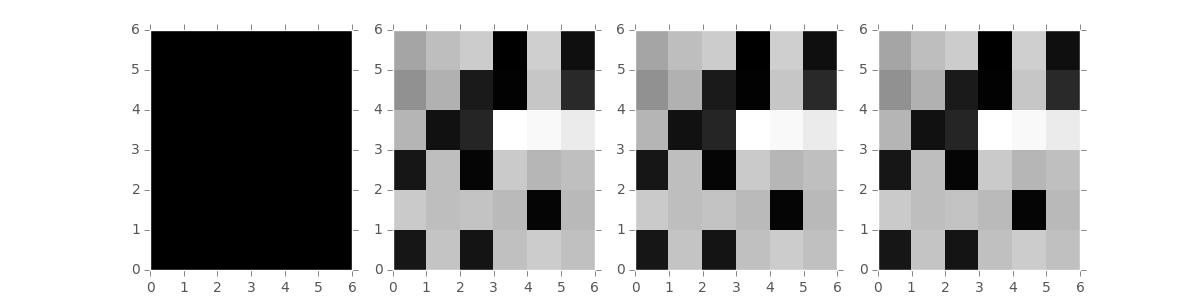
\includegraphics[width=\linewidth]{data_files/detected_total_features.png}
\caption {Features possesed by each image in the data}
\label{fig:da}
\end{figure}

\begin{table}[ht]
\centering
\caption{Presence of original features \label{featu}}
\begin{tabular}{lrrrr}
\toprule
{} &  F1 &  F2 &  F3 &  F4 \\
\midrule
1st image &   0 &   1 &   0 &   0 \\
2nd image &   1 &   1 &   0 &   0 \\
3rd image &   1 &   1 &   0 &   1 \\
4th image &   1 &   1 &   0 &   0 \\
\bottomrule
\end{tabular}

\end{table}

\begin{figure}
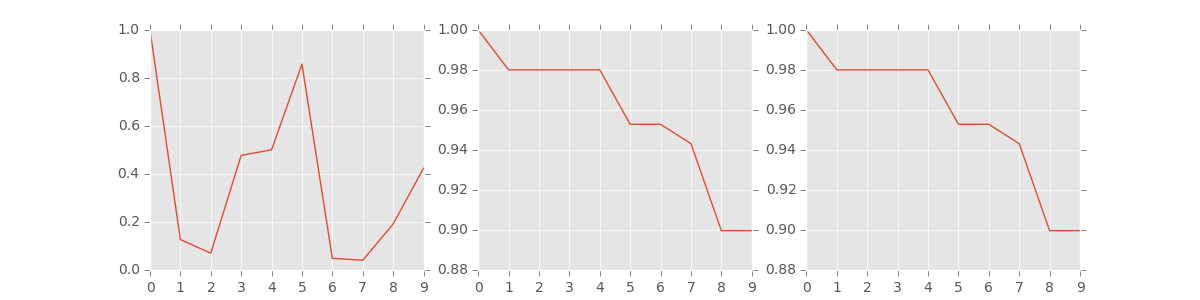
\includegraphics[width=\linewidth]{data_files/trace_plots.png}
\caption {Trace plots for alpha, original sigma X and original sigma alpha}
\label{fig:da}
\end{figure}


\end{document}